\documentclass[tikz, convert={outext=.svg,pdf2svg}]{standalone}

\usepackage{tikz,amsmath,amssymb,bm,color}
\usetikzlibrary{shapes,arrows,calc,backgrounds,decorations.pathreplacing}

\definecolor{myblue}{RGB}{175, 204, 233}

\begin{document}
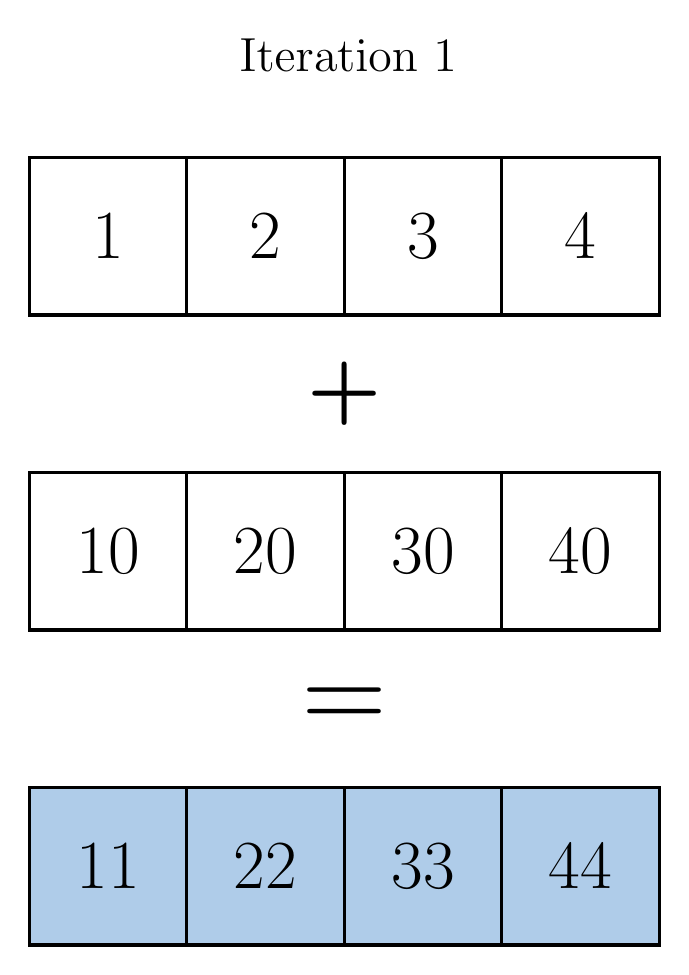
\begin{tikzpicture}

\tikzstyle{square} = [draw,outer sep=5,inner sep=3,minimum size=10,
    line width=0, very thick, draw=black!100,
    top color=white,bottom color=white]
\tikzstyle{blue} = [draw=black,outer sep=0,inner sep=0,line width=1,
    very thick, minimum width=2cm, minimum height=2cm, 
    top color=myblue, bottom color=myblue, font=\Huge, align=center]

% =========================
% four scalars - first row (flush)
% =========================
\draw[square] (9,10.5) rectangle (11,12.5);
\node at (10,11.5) {\Huge 1};
\node[scale=1.2] at (13.05,13.8) {\Large Iteration 1};

\draw[square] (11,10.5) rectangle (13,12.5);
\node at (12,11.5) {\Huge 2};


\draw[square] (13,10.5) rectangle (15,12.5);
\node at (14,11.5) {\Huge 3};


\draw[square] (15,10.5) rectangle (17,12.5);
\node at (16,11.5) {\Huge 4};


% =========================
% four scalars - second row (flush)
% =========================
\draw[square] (9,6.5) rectangle (11,8.5);
\node at (10,7.5) {\Huge 10};

\draw[square] (11,6.5) rectangle (13,8.5);
\node at (12,7.5) {\Huge 20};

\draw[square] (13,6.5) rectangle (15,8.5);
\node at (14,7.5) {\Huge 30};

\draw[square] (15,6.5) rectangle (17,8.5);
\node at (16,7.5) {\Huge 40};

% plus signs between vector 1 and vector 2

\node[scale=3] at (13.0,9.5) {\textbf{+}};



% =========================
% Down arrows
% =========================

\node[scale=4] at (13,5.5) {$=$};



% =========================
% four scalars - results (flush, blue style)
% =========================
\node[blue] at (10,3.5) {11};
\node[blue] at (12,3.5) {22};
\node[blue] at (14,3.5) {33};
\node[blue] at (16,3.5) {44};

\end{tikzpicture}
\end{document}

